
\chapter{Arquitetura de Software}
\label{sec-arquitetura}
\vspace{-1cm}

A Figura~\ref{figura-arquitetura} mostra a arquitetura do sistema \emph{\imprimirtitulo}.

\begin{figure}[h]
	\centering
	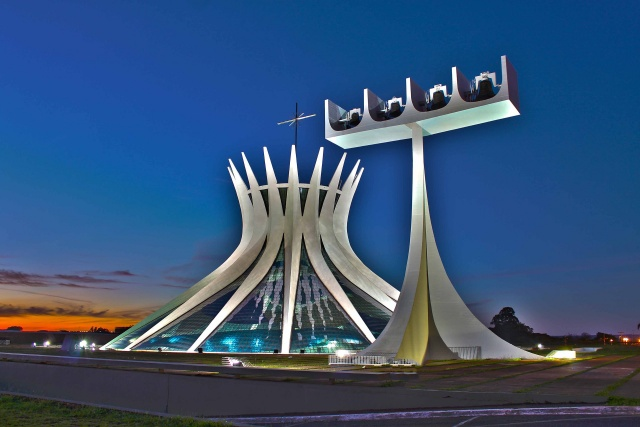
\includegraphics[width=0.8\textwidth]{figuras/figura-arquitetura}
	\caption{Arquitetura do sistema.}
	\label{figura-arquitetura}
\end{figure}

\vitor{Substituir a Figura~\ref{figura-arquitetura} pelo diagrama UML da arquitetura do seu projeto e descrevê-la no texto. Caso use alguma arquitetura clássica, incluir referência bibliográfica com BibTeX (ex.:Camada de Serviço~\cite{fowler:book02}). Como exemplo, vide documentos de projeto do Marvin e da Locadora de Carros do prof. Ricardo Falbo.}
